\chapter{Estimativa da fase transiente}
\label{chap:estimativa}

Os valores usados para a fase transiente de cada experimento foram estimados desenhando gráficos mostrando a geração dos valores da variância do tempo de espera na fila 2 (V(W2)) em 5 rodadas.

Esse estimador foi usado pois ele é o que converge mais lentamente para o intervalo de confiança válido. Este fato foi comprovado executando o simulador um número considerável de vezes para cada tipo de utilização do servidor.

Foram gerados diversos gráficos para cada utilização, e em cada um deles a semente é diferente, já que ela é definida como está exposto na seção \ref{sec:random}. Todos mostraram o mesmo comportamento. Escolhemos um de cada tipo de experimento para mostrar no relatório.

Com os gráficos gerados foi possível ter uma boa noção de que em que ponto o simulador começa a entrar na fase de equilíbrio. Eles são mostrados na seção \ref{sec:graficos}.

\section{No simulador}

Dentro do simulador esses valores de fase transiente para cada experimento são dados em uma lista junto com os valores das taxas de entrada.

\section{Gráficos}
\label{sec:graficos}

\begin{figure}[htb!]
   \subfloat[First Come First Served]{\label{fig:p2FCFS}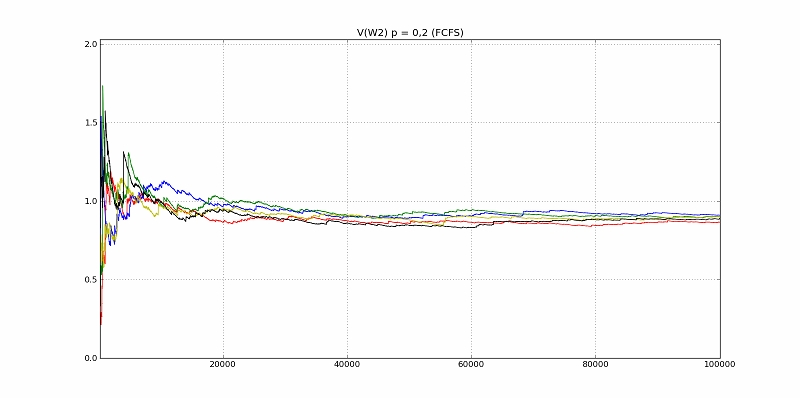
\includegraphics[width=1.0\textwidth]{V[W2]p=0_2FCFS.jpg}}\\
   \subfloat[Last Come First Served]{\label{fig:p2LCFS}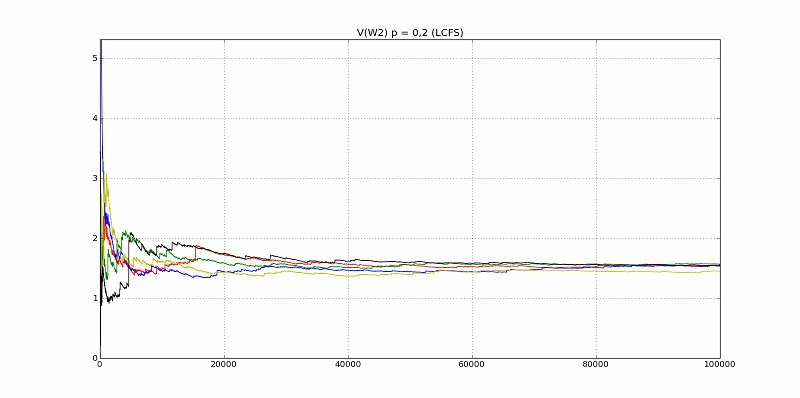
\includegraphics[width=1.0\textwidth]{V[W2]p=0_2LCFS.jpg}}
   \caption{V(W2) para $\rho=0.2$. Nesse caso identificamos que a fase de equilíbrio começa quando aproximadamente 30.000 clientes já passaram pelo sistema.}
\end{figure}

\begin{figure}[htb!]
   \subfloat[First Come First Served]{\label{fig:p4FCFS}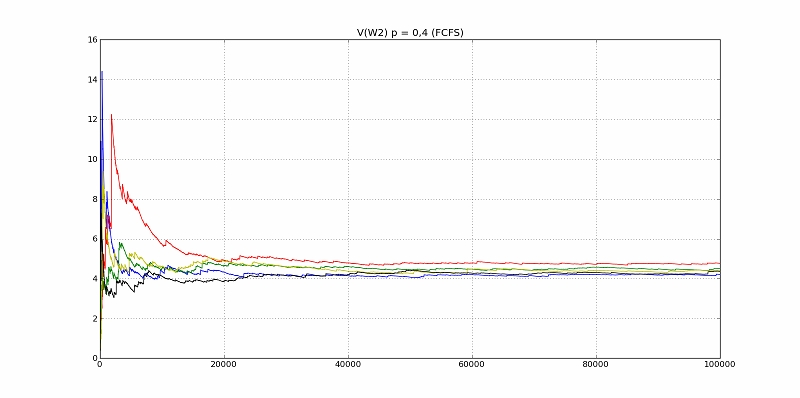
\includegraphics[width=1.0\textwidth]{V[W2]p=0_4FCFS.jpg}}\\
   \subfloat[Last Come First Served]{\label{fig:p4LCFS}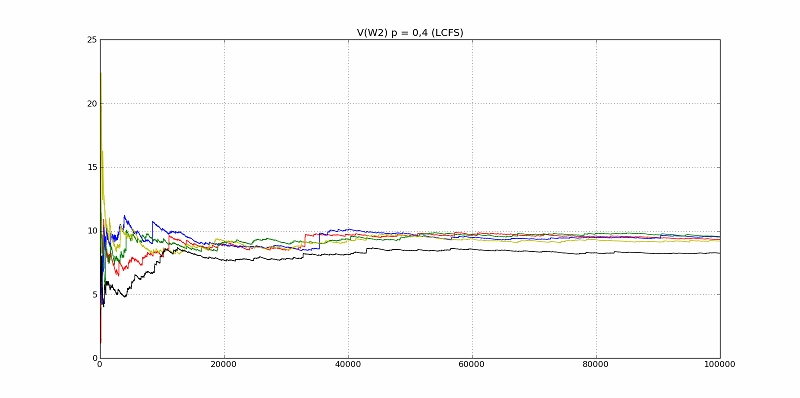
\includegraphics[width=1.0\textwidth]{V[W2]p=0_4LCFS.jpg}}
   \caption{V(W2) para $\rho=0.4$. Nesse caso identificamos que a fase de equilíbrio começa quando aproximadamente 40.000 clientes já passaram pelo sistema.}
\end{figure}

\begin{figure}[htb!]
   \subfloat[First Come First Served]{\label{fig:p6FCFS}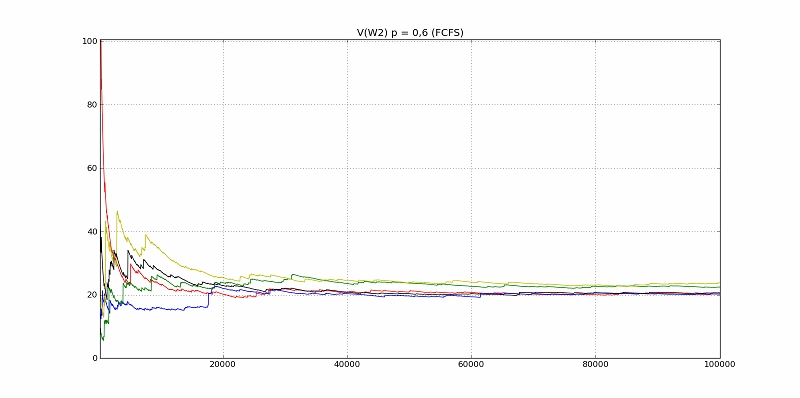
\includegraphics[width=1.0\textwidth]{V[W2]p=0_6FCFS.jpg}}\\
   \subfloat[Last Come First Served]{\label{fig:p6LCFS}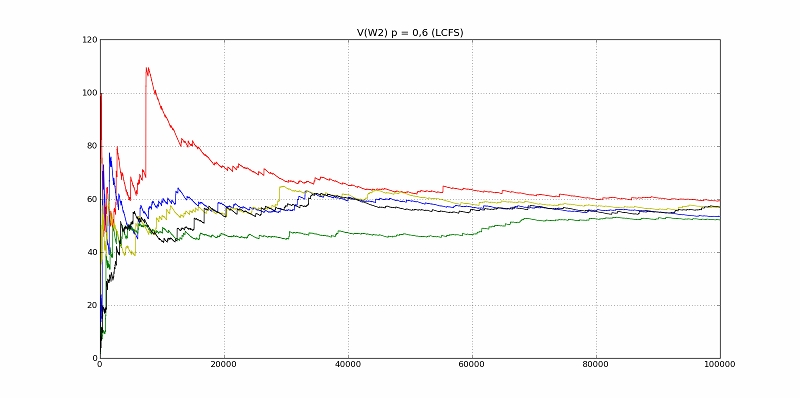
\includegraphics[width=1.0\textwidth]{V[W2]p=0_6LCFS.jpg}}
   \caption{V(W2) para $\rho=0.6$. Nesse caso identificamos que a fase de equilíbrio começa quando aproximadamente 80.000 clientes já passaram pelo sistema.}
\end{figure}

\begin{figure}[htb!]
   \subfloat[First Come First Served]{\label{fig:p8FCFS}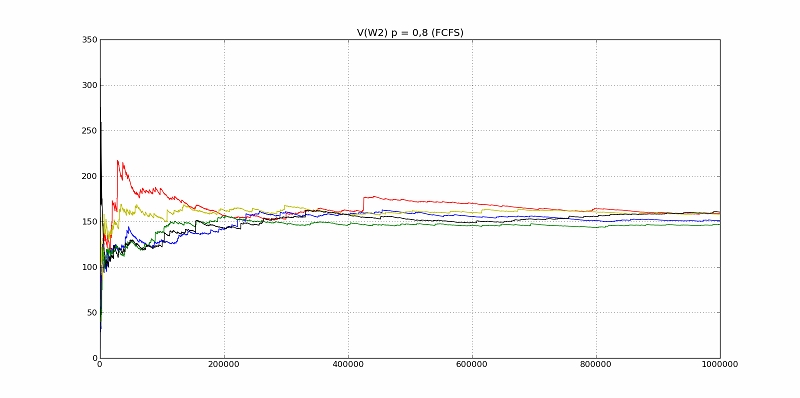
\includegraphics[width=1.0\textwidth]{V[W2]p=0_8FCFS.jpg}}\\
   \subfloat[Last Come First Served]{\label{fig:p8LCFS}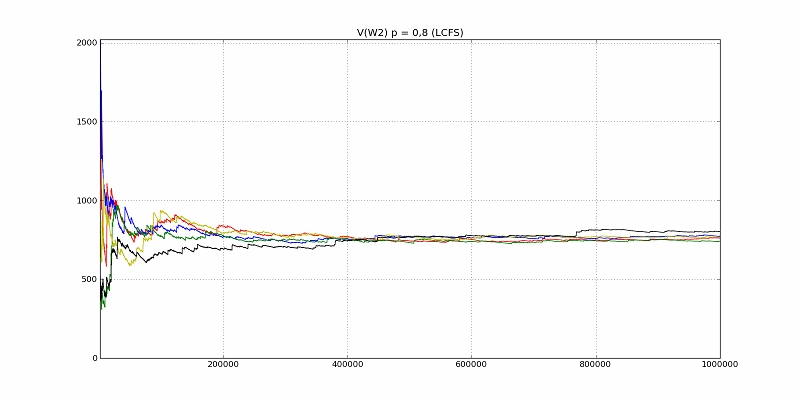
\includegraphics[width=1.0\textwidth]{V[W2]p=0_8LCFS.jpg}}
   \caption{V(W2) para $\rho=0.8$. Nesse caso identificamos que a fase de equilíbrio começa quando aproximadamente 400.000 clientes já passaram pelo sistema.}
\end{figure}

\begin{figure}[htb!]
   \subfloat[First Come First Served]{\label{fig:p9FCFS}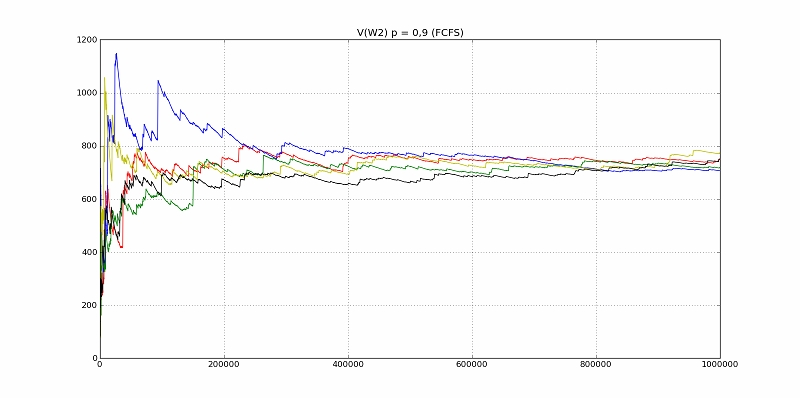
\includegraphics[width=1.0\textwidth]{V[W2]p=0_9FCFS.jpg}}\\
   \subfloat[Last Come First Served]{\label{fig:p9LCFS}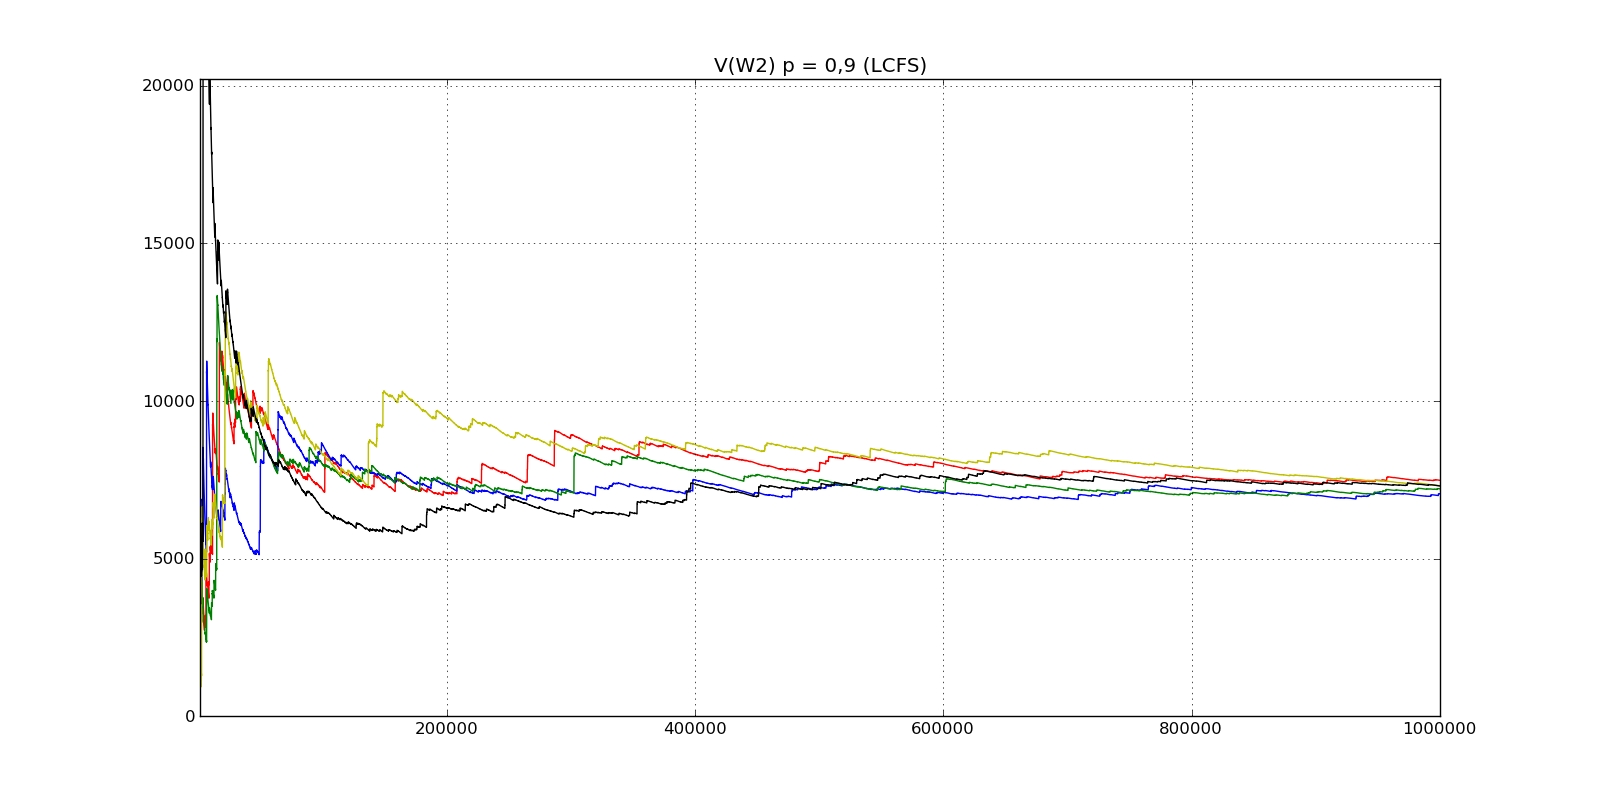
\includegraphics[width=1.0\textwidth]{V[W2]p=0_9LCFS.jpg}}
   \caption{V(W2) para $\rho=0.9$. Nesse caso identificamos que a fase de equilíbrio começa quando aproximadamente 500.000 clientes já passaram pelo sistema.}
\end{figure}